\chapter{Introduction}

This thesis presents measurements of W and Z vector boson production, 
decaying leptonically and associated
with two forward and high momentum jets, produced in proton-proton (pp) collisions
at the CERN Large Hadron Collider (LHC). 
The contribution to this process dominated by fully electroweak (EW)
interactions, which includes direct couplings of the W and Z bosons, 
is extracted and measured with an observed significance of
1.9 standard deviations, with 2.7 standard deviations expected. 
This is the first measurement of this process at CMS. 

The presence and production rate of the \EWWZ process is intimately connected to the 
phenomenon of EW symmetry breaking (EWSB) \cite{Quigg:2009vq}, which gives rise to masses of
the vector bosons and their self-interactions. A fundamental prediction
of EWSB, fulfilled in the SM by the Brout-Englert-Higgs (BEH) mechanism,
is the emergence of a scalar particle, referred 
to as the Higgs boson. 
This particle was first observed by the 
ATLAS~\cite{Aad:2012tfa} and CMS~\cite{Chatrchyan:2012xdj,Chatrchyan:2013lba} Collaborations
at CERN in 2012, providing compelling evidence for the BEH mechanism as
a component of the SM theory.

Given the Higgs boson mass, the self-interactions 
of the W and Z bosons are precisely predicted in the SM. 
An excess of \EWWZ events with respect to the SM prediction could indicate contributions from 
additional gauge boson or vector resonances~\cite{Delgado:2017cls}, 
additional Higgs or scalar bosons~\cite{Kilian:2015opv}, 
or it could suggest that the gauge or Higgs bosons are not elementary~\cite{Csaki:2015hcd}.
Measurements of this process can thus be used to constrain the predictions
of such beyond the SM (BSM) theories. 

This thesis presents constraints on BSM physics predicted by explicit models
including charged Higgs bosons 
and in the generalized framework of dimension-8 effective field theory (EFT) operators.
Constraints on the masses and couplings strengths of a hypothetical
charged Higgs boson presented here extend the previous CMS results~\cite{Sirunyan:2017sbn}, and
are complementary to those recently presented by the ATLAS Collaboration~\cite{Aaboud:2018ohp}. 
These results suggest that EWSB is uniquely fulfilled by the SM Higgs boson,
or that additional partners must be of significantly higher mass than the
SM Higgs boson.
Constraints on EFT operators provide limitations on a broad class of new physics
models, and can be interpreted in terms of a minimum energy scale at which additional
interactions than those predicted by the SM are feasible.
These results are the first constraints on dimension-8 EFT operators 
in from pp collisions with center of mass energy of 13 TeV in the WZ channel.

This study follows the first observations of EW diboson production
by the ATLAS~\cite{ATLAS-CONF-2018-030,ATLAS-CONF-2018-033} and CMS~\cite{Sirunyan:2017ret} Collaborations
and establishes \EWWZ production as an important
probe of precision calculations in the SM while extending its importance 
in the search for New Physics.
All measurements presented are consistent with the standard model predictions,
providing support for the modern techniques for predictions concerning LHC collisions, and 
increasing evidence that the Higgs boson is the unique medium of EWSB 
at the energy scale probed by the 13 TeV LHC.

\section{The universe of particles}

The idea of understanding the physical world by identifying its
fundamental constituents is a very old one. Ancient eastern and
western philosophers independently attempted the feat, concluding
independently that the world could be reduced 
to ``elements'' such as water, earth, and fire.
As modern thought began to develop observational science, 
evidence mounted that these elements themselves were 
not indivisible. Perhaps the Greeks had not identified
the correct fundamental elements, but the belief that this endeavor could
be accomplished lived on.

A major attraction of identifying the fundamental constituents 
is its implications for constructing a macroscopic description from these
pieces. This process of understanding a complex system through is pieces, 
termed ``reductionism'' by philosophers, has enjoyed
many moments of triumph throughout history, 
In practice, the step from the fundamental to the macroscopic 
is far from trivial. Despite a well-established
understanding of the proton constituents and their interactions,
predicting the proton mass from first principles has only recently 
been achieved~\cite{Durr:2008zz}, and larger systems remain well
out of reach.
In addition to the challenges of calculability, additional structures
may arise from the nature of large systems, such as ferromagnetism or 
superconductivity.
This long-accepted path to a complete description of the physical world
has thus rightly been called into question, and it may never be feasible
to achieve a theory of biology built from the findings of particle 
physics~\cite{Anderson393}.
Yet there is an undeniable elegance in achieving a concise description
of the fundamental elements of the natural world and their interactions,
and this remains the target of the field of particle physics today. 

The modern genesis of the field can perhaps be credited to 
the discovery of the electron in 1897 by J. J. Thomson.
The electromagnetic interactions of this particle had been 
already been described by James Clerk Maxwell decades earlier.
The turn of the century began a saw an explosion in the theoretical
understanding of the 

\section{Particle collider experiments}

To observe the smallest pieces of matter, one must break matter into pieces.
The discovery of radioactivity in the late 1800s by Henri Becquerel had
profound implications for this idea, as it represented the spontaneous
disintegration of atoms into smaller pieces.

Studies of cosmic rays followed shortly afterwards, a


Be

Cosmic ray experiments
Transition from cosmic rays to colliders
Crockoff and Walton

Move very quickly up to collider experiment, especially LEP,
the Tevatron, and the LHC
\section{Motivation and context of this result}
The work presented in this thesis
has two related motivations: performing a measurement of a rare
process predicted by the standard model, and searching for signs of 
BSM physics in a channel and topology not previously probed at the 13 TeV LHC.
Previous studies have laid the groundwork for these interpretations.

Characterizing the self-interactions of the vector bosons is in important
step to understanding the self-consistency of the SM, and a useful probe
of possible deviations from its predictions. Because the production of events
with multiple vector bosons in the final state
requires collisions with a high center of mass energy, the LHC has
exceeded previous measurements of these processes.

Measurements WW and WW$\gamma$ production in electron--positron collisions
were first made at the LEP
Collider at CERN by the ALEPH, DELPHI, L3, and OPAL Collaborations~\cite{LEP-2}.
These processes are sensitive to the triple vector boson couplings
WWZ and WW$\gamma$, and the quartic couplings WW$\gamma\gamma$
and WWZ$\gamma$. The production rate and angular distributions of the decay
products of the vector bosons in these states were used to derive values 
of the triple and quartic couplings. No deviations were observed from the 
predictions of the SM with a light Higgs boson.

Production of charged vector boson pairs was also studied in proton--antiproton
collisions at the Tevatron Collider at the Fermi National Accelerator Laboratory
in Illinois. The measurement of WZ production, inclusive in the
number of clustered hadronic particles -- referred to as jets, was
first performed by the CDF~\cite{Aaltonen:2012vu,Abulencia:2007tu} 
and D0~\cite{Abazov:2012cj} Collaborations at the Tevatron in 2006. 
Measurements of the WWZ coupling were found to be consistent with the results
from the LEP experiments and with the SM.
Experimental sensitivity to quartic couplings of the massive vector boson 
was first achieved at the LHC.

\begin{figure}[htbp]
  \centering
   \subfigure[]{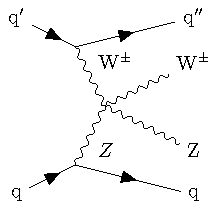
\includegraphics[page=1,width=0.2\textwidth]{figures/FeynmanDiagrams/feynmanVBS.pdf}}\qquad
   \subfigure[]{\includegraphics[page=2,width=0.2\textwidth]{figures/FeynmanDiagrams/feynmanVBS.pdf}}\qquad
   \subfigure[]{\includegraphics[page=3,width=0.2\textwidth]{figures/FeynmanDiagrams/feynmanVBS.pdf}}\qquad
   \subfigure[]{\includegraphics[page=4,width=0.2\textwidth]{figures/FeynmanDiagrams/feynmanVBS.pdf}}\qquad
  \caption{Representative Feynman diagrams for \WZjj production in the SM and BSM. 
  EW-induced WZ production includes quartic interactions (a) of the vector bosons.
  This is distinguishable from QCD-induced production (b) through kinematic variables.
  New physics in the EW sector modifying the quartic coupling 
  can be parameterized in terms of dimension-eight effective field theory operators (c).
  Specific models modifying this interaction include those predicting charged Higgs bosons (d).
  }
 \label{fig:feynmanDiagrams}
\end{figure}

The total \WZ production cross section in proton--proton collisions 
has been measured in the leptonic decay modes by the CMS and ATLAS collaboration at 
7, 8 and 13 TeV~\cite{Aad:2012twa,Aad:2016ett,Khachatryan:2016tgp,Khachatryan:2016poo}, 
and limits on anomalous triple gauge couplings were presented in Refs.~\cite{Aad:2016ett,Khachatryan:2016poo}. 
Constraints on anomalous quartic gauge couplings (aQGC) were presented by the ATLAS collaboration at 8 TeV~\cite{Aad:2016ett}. 
At the LHC, quartic WZ interactions are accessible through triple vector boson production or through vector boson scattering (VBS), 
in which vector bosons are radiated from the incoming quarks before interacting.
These interactions include WZ quartic couplings, as shown in Fig.~\ref{fig:feynmanDiagrams}~(a). 
VBS processes form a distinct experimental signature characterized by two forward and high momentum jets in addition 
to the vector bosons. They are part of an important subclass of processes contributing to 
\WZ plus two jet (\WZjj) production that proceeds entirely via the EW interaction at tree level,
$\mathcal{O}(\alpha^4)$, which we refer to as EW-induced \WZjj production, or simply \EWWZ production. 
An additional contribution to the \WZjj state proceeds via QCD radiation of partons from 
the incoming quark or gluon lines, shown in Fig.~\ref{fig:feynmanDiagrams}~(b), 
leading to contributions at $\mathcal{O}(\alpha^2\alpha_{S}^2)$.
This class of processes is referred to as QCD-induced WZjj production (or \QCDWZ),
and is distinguishable from the EW-induced component via kinematic variables.

In the SM, EWSB is fulfilled by a single Higgs field, which transforms as an SU$(2)_{L}$ doublet.
Extending the Higgs sector by at least one additional SU$(2)_{L}$ doublet leads necessarily
to additional charged scalar particles. An extended Higgs sector is predicted by many
complex BSM theories, including the Minimal Supersymmetric SM. As a general
search, establishing if the Higgs sector of the SM is interesting.

Searches for charged Higgs bosons were carried out in detail at the LEP Collider~\cite{}.

This work is the best.

\section{Overview}

The outline of this work is as follows: chapter 2 presents an extended 
overview of the theoretical underpinnings of this work, including the foundations
of the SM and the role of \EWWZ production in this framework. The motivations 
and structure of SM extensions probed in this work are also introduced.
Chapter 3 introduces the experimental setup and apparatus used to study W and 
Z boson production in the laboratory. The LHC and the Compact Muon Solenoid 
detector are presented and discussed. Chapter 4 describes the procedure of 
building predictions for vector boson production in pp collisions.
The use of these predictions in interpreting results, and in developing simulation
of particle production and decays in pp collisions, and their susequent interactions
with the detector, which is used 
guide the analysis approach and optimizations, are discussed. Chapter 5 presents
the process of finding particle candidates from electronic signals in the detector.
Chapter 6 details the procedure of this analysis and the statistical underpinnings
used to extract results. Chapter 7 discuesses the results obtained from this study
and discusses their interpretations and implications. Chapter 8 summarizes the
results presented and discusses future extensions.
